\documentclass[14pt]{extreport}
\usepackage{gost}
%\usepackage{hyperref}
%\usepackage{makecell}
\usepackage{ragged2e}
%\usepackage{graphicx}%Вставка картинок правильная
%\usepackage{float}%"Плавающие" картинки
%\usepackage{wrapfig}%Обтекание фигур (таблиц, картинок и прочего)
%\justifying
\makeatletter
\@addtoreset{figure}{part}% Reset figure numbering at every part
\makeatother
\renewcommand{\thefigure}{\arabic{figure}}% Figure number is part.figure
\renewcommand{\thetable}{\arabic{table}}

%Тут можно вставить дополнительные пакеты

\begin{document}
    \pagestyle{empty} %  выключаем нумерацию
    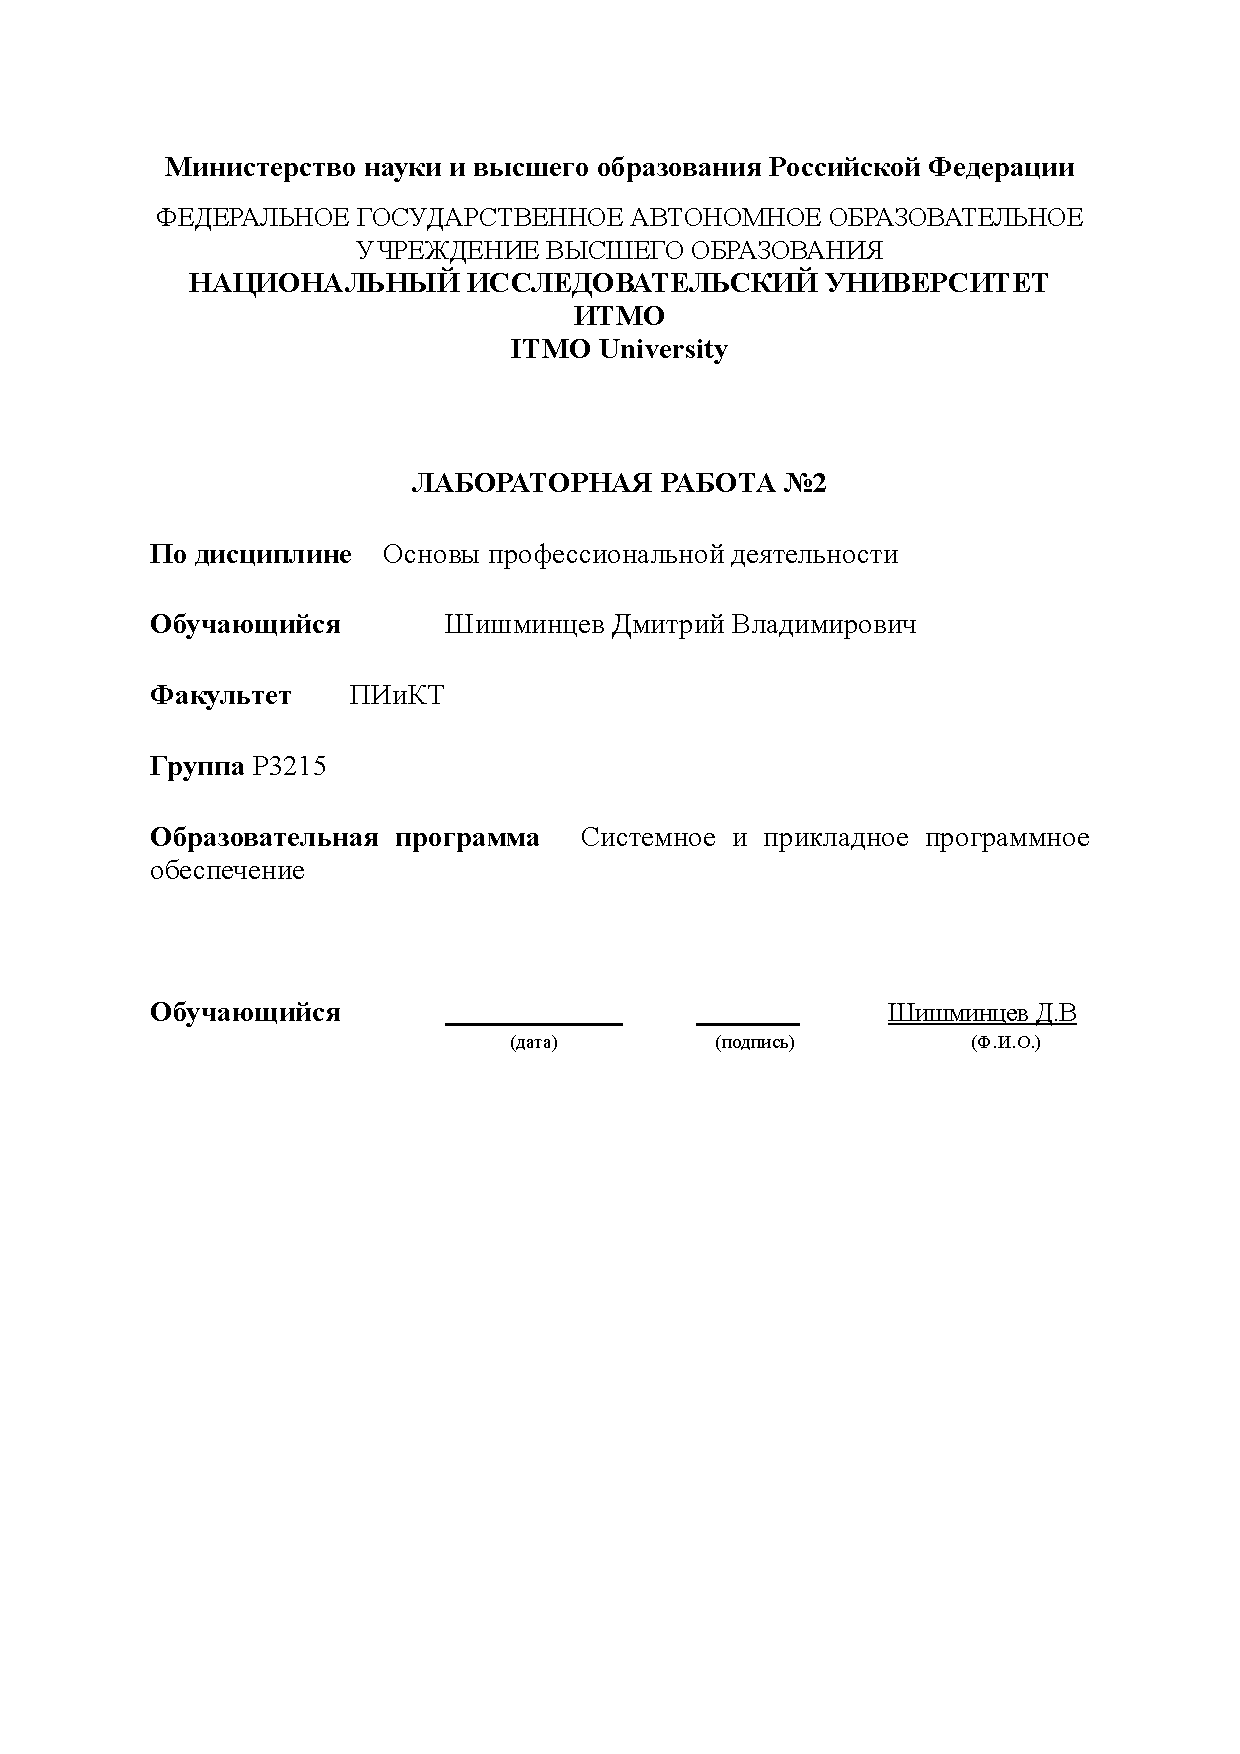
\includepdf[pages=-,pagecommand={}]{title_page.pdf}

    \pagestyle{plain} % включаем нумерацию
    \tableofcontents
    \intro

    Задание по базовой электронной вычислительной машине (ЭВМ) предполагает анализ программы, определение её функции, области представления и области допустимых значений исходных данных и результатов. В процессе выполнения задания требуется также провести трассировку программы и предложить вариант с уменьшенным числом команд. Этот анализ поможет понять, как программа взаимодействует с данными и как можно оптимизировать её выполнение.


    \chapter{Текст задания}
        По выданному преподавателем варианту определить функцию, вычисляемую программой, область представления и область допустимых значений исходных данных и результата, выполнить трассировку программы, предложить вариант с меньшим числом команд. При выполнении работы представлять результат и все операнды арифметических операций знаковыми числами, а логических операций набором из шестнадцати логических значений.

        \begin{figure}[!h]
            \centering
            
\includegraphics[width=0.4\linewidth]{img.png}
            \caption{Картинка задания}

        \end{figure}


    \chapter{Таблица исходной программы}
        \begin{table}[h]

            \centering
            \begin{tabular}{|c|c|c|c|}
                \hline
                Адрес & Код команды & Мнемоника & Комментарий \\
                \hline
                058    &    4070    &     & Исходная переменная (a)\\ \hline
                059    &    3071    &     & Результирующая переменная \\ \hline
                \hline
                05A    &    0200    &   CLA         & 0 => AC \\ \hline
                05B    &    4072    &   ADD    072  & AC + 072 => AC \\ \hline
                05C    &    6058    &   SUB    058  & AC - 058 => AC \\ \hline
                05D    &    E070    &   ST     070  & AC => 070 \\ \hline
                05E    &    A073    &   LD     073  & 073 => AC \\ \hline
                05F    &    2070    &   AND    070  & AC AND 070 => AC \\ \hline
                060    &    E070    &   ST     070  & AC => 070 \\ \hline
                061    &    0200    &   CLA         & 0 => AC \\ \hline
                062    &    606F    &   SUB    06F  & AC - 06F => AC \\ \hline
                063    &    4070    &   ADD    070  & AC + 070 => AC \\ \hline
                064    &    E070    &   ST     070  & AC => 070 \\ \hline
                065    &    0200    &   CLA         & 0 => AC \\ \hline
                066    &    3071    &   OR     071  & AC OR 071 => AC \\ \hline
                067    &    3070    &   OR     070  & AC OR 070 => AC \\ \hline
                068    &    E070    &   ST     070  & AC => 070 \\ \hline
                069    &    0200    &   CLA         & 0 => AC \\ \hline
                06A    &    606E    &   SUB    06E  & AC - 06E => AC \\ \hline
                06B    &    4070    &   ADD    070  & AC + 070 => AC \\ \hline
                06C    &    E059    &   ST     059  & AC => 059 \\ \hline
                06D    &    0100    &   HLT         & Завершение программы \\ \hline
                \hline
                06E    &    E070    &     & Исходная переменная (b)\\ \hline
                06F    &    A073    &     & Исходная переменная (c)\\ \hline
                070    &    3070    &     & Переменная для промежуточного значения \\ \hline
                071    &    E070    &     & Исходная переменная (d)\\ \hline
                072    &    0200    &     & Исходная переменная (e)\\ \hline
                073    &    6058    &     & Исходная переменная (f)\\ \hline


            \end{tabular}\label{tab:table}
        \end{table}

    \chapter{Анализ исходной программы}
    \section{Реализуемая функция}
            Исходная программа реализует вычисление функции:

            $$F(a, b, c, d, e, f) = (((e-a) AND (f-c)) OR (d)) - b $$
    \section{Область представления информации}
        $e, a, f, c, b$ - 16ти разрядные знаковые числа


        $b $ - 16ти разрядная логическая переменаня
    \section{Область допустимых значений}
            \subsection*{Случай 1 - ограничение разрядности:}
                \begin{cases}
                    2^{14} <= e, a, f, c, b <= 2^{14} -1 \\
                    d_{14} = 0
                \end{cases}
            \subsection*{Случай 2:}
                \begin{cases}
                    2^{14} <= e <= 2^{15} -1 \\
                    0 <= a <= 2^{15} - 1 \\
                    -2^{15} <= e <= 2^{14} - 1 \\
                    -2^{15} <= a <= 0 \\
                    d_{15} = 0 \\
                    -2^{15} <= b <= 0
                \end{cases}

            \subsection*{Случай 3:}
                \begin{cases}
                    2^{14} <= e <= 2^{15} -1 \\
                    0 <= a <= 2^{15} - 1 \\
                    -2^{15} <= f <= 2^{14} - 1 \\
                    -2^{15} <= c <= 0 \\
                    d_{15} = 0 \\
                    -2^{15} <= b <= 0
                \end{cases}

            \subsection*{Случай 4:}
                \begin{cases}
                    -2^{15} <= e <= 2^{14} - 1 \\
                    -2^{15} <= a <= 0 \\
                    2^{14} <= f <= 2^{15} -1 \\
                    0 <= c <= 2^{15} - 1
                    d_{15} = 0 \\
                    -2^{15} <= b <= 0
                \end{cases}

            \subsection*{Случай 5:}
                \begin{cases}
                    -2^{15} <= e <= 2^{14} - 1 \\
                    -2^{15} <= a <= 0 \\
                    -2^{15} <= f <= 2^{14} - 1 \\
                    -2^{15} <= c <= 0 \\
                    d_{15} = 0 \\
                    -2^{15} <= b <= 0
                \end{cases}

            \subsection*{Случай 6:}
                \begin{cases}
                    2^{14} <= e <= 2^{15} -1 \\
                    0 <= a <= 2^{15} - 1 \\
                    -2^{15} <= e <= 2^{14} - 1 \\
                    -2^{15} <= a <= 0 \\
                    d_{15} = 1 \\
                    0 <= b <= 2^{15} - 1
                \end{cases}

            \subsection*{Случай 7:}
                \begin{cases}
                    2^{14} <= e <= 2^{15} -1 \\
                    0 <= a <= 2^{15} - 1 \\
                    -2^{15} <= f <= 2^{14} - 1 \\
                    -2^{15} <= c <= 0 \\
                    d_{15} = 1 \\
                    0 <= b <= 2^{15} - 1
                \end{cases}

            \subsection*{Случай 8:}
                \begin{cases}
                    -2^{15} <= e <= 2^{14} - 1 \\
                    -2^{15} <= a <= 0 \\
                    2^{14} <= f <= 2^{15} -1 \\
                    0 <= c <= 2^{15} - 1
                    d_{15} = 1 \\
                    0 <= b <= 2^{15} - 1
                \end{cases}

            \subsection*{Случай 9:}
                \begin{cases}
                    -2^{15} <= e <= 2^{14} - 1 \\
                    -2^{15} <= a <= 0 \\
                    -2^{15} <= f <= 2^{14} - 1 \\
                    -2^{15} <= c <= 0 \\
                    d_{15} = 1 \\
                    0 <= b <= 2^{15} - 1
                \end{cases}


%            \begin{cases}
%                2^{14} <= e <= 2^{15} -1 \\
%                0 <= a <= 2^{15} - 1
%            \end{cases}
%
%            \begin{cases}
%                -2^{15} <= e <= 2^{14} - 1 \\
%                -2^{15} <= a <= 0
%            \end{cases}
%
%            \begin{cases}
%                2^{14} <= f <= 2^{15} -1 \\
%                0 <= c <= 2^{15} - 1
%            \end{cases}
%
%            \begin{cases}
%                -2^{15} <= f <= 2^{14} - 1 \\
%                -2^{15} <= c <= 0
%            \end{cases}


    \section{Расположение в памяти ЭВМ}

        Адреса исполняемых команд: 05A-06D

        Адреса исходных данных: 058, 059, 06E-073

        \begin{landscape}
            \chapter{Трассировка программы}
            \begin{table}[!h]
                \centering
                \begin{tabular}{|l|l|l|l|l|l|l|l|l|l|l|l|l|}
                    \hline
                    Адр & Знчн & IP & CR & AR & DR & SP & BR & AC & PS & NZVC & Адр & Знчн \\ \hline
                    05A & 0200 & 05A & 0000 & 000 & 0000 & 000 & 0000 & 0000 & 004 & 0100 & ~ & ~ \\ \hline
                    05A & 0200 & 05B & 0200 & 05A & 0200 & 000 & 005A & 0000 & 004 & 0100 & ~ & ~ \\ \hline
                    05B & 4072 & 05C & 4072 & 072 & 0200 & 000 & 005B & 0200 & 000 & 0000 & ~ & ~ \\ \hline
                    05C & 6058 & 05D & 6058 & 058 & 4070 & 000 & 005C & C190 & 008 & 1000 & ~ & ~ \\ \hline
                    05D & E070 & 05E & E070 & 070 & C190 & 000 & 005D & C190 & 008 & 1000 & 070 & C190 \\ \hline
                    05E & A073 & 05F & A073 & 073 & 6058 & 000 & 005E & 6058 & 000 & 0000 & ~ & ~ \\ \hline
                    05F & 2070 & 060 & 2070 & 070 & C190 & 000 & 005F & 4010 & 000 & 0000 & ~ & ~ \\ \hline
                    060 & E070 & 061 & E070 & 070 & 4010 & 000 & 0060 & 4010 & 000 & 0000 & 070 & 4010 \\ \hline
                    061 & 0200 & 062 & 0200 & 061 & 0200 & 000 & 0061 & 0000 & 004 & 0100 & ~ & ~ \\ \hline
                    062 & 606F & 063 & 606F & 06F & A073 & 000 & 0062 & 5F8D & 000 & 0000 & ~ & ~ \\ \hline
                    063 & 4070 & 064 & 4070 & 070 & 4010 & 000 & 0063 & 9F9D & 00A & 1010 & ~ & ~ \\ \hline
                    064 & E070 & 065 & E070 & 070 & 9F9D & 000 & 0064 & 9F9D & 00A & 1010 & 070 & 9F9D \\ \hline
                    065 & 0200 & 066 & 0200 & 065 & 0200 & 000 & 0065 & 0000 & 004 & 0100 & ~ & ~ \\ \hline
                    066 & 3071 & 067 & 3071 & 071 & E070 & 000 & 1F8F & E070 & 008 & 1000 & ~ & ~ \\ \hline
                    067 & 3070 & 068 & 3070 & 070 & 9F9D & 000 & 0002 & FFFD & 008 & 1000 & ~ & ~ \\ \hline
                    068 & E070 & 069 & E070 & 070 & FFFD & 000 & 0068 & FFFD & 008 & 1000 & 070 & FFFD \\ \hline
                    069 & 0200 & 06A & 0200 & 069 & 0200 & 000 & 0069 & 0000 & 004 & 0100 & ~ & ~ \\ \hline
                    06A & 606E & 06B & 606E & 06E & E070 & 000 & 006A & 1F90 & 000 & 0000 & ~ & ~ \\ \hline
                    06B & 4070 & 06C & 4070 & 070 & FFFD & 000 & 006B & 1F8D & 001 & 0001 & ~ & ~ \\ \hline
                    06C & E059 & 06D & E059 & 059 & 1F8D & 000 & 006C & 1F8D & 001 & 0001 & 059 & 1F8D \\ \hline
                    06D & 0100 & 06E & 0100 & 06D & 0100 & 000 & 006D & 1F8D & 001 & 0001 & ~ & ~ \\ \hline
                \end{tabular}
            \end{table}
        \end{landscape}

    \chapter{Вариант с наименьшим количество команд}
    \begin{verbatim}
    CLA
    ADD 072
    SUB 058
    ST 070
    LD 073
    AND 070
    SUB 06f
    OR 071
    SUB 06e
    ST 059
        \end{verbatim}
    \conclusions

        Исследование программы на базовой ЭВМ позволяет глубже понять её работу и оптимизировать выполнение, что важно для повышения эффективности и экономии ресурсов. Анализ функции, области представления и области допустимых значений данных, трассировка программы и оптимизация команд помогут более эффективно использовать ресурсы ЭВМ и достичь более эффективных результатов в вычислениях.
\end{document}